\documentclass[11pt,a4paper,english]{article}
\usepackage[english]{babel}
\usepackage[utf8]{inputenc}
\usepackage{amsmath,amsfonts,amssymb,graphicx,textcomp,caption,color,listings,subcaption}
\usepackage[T1]{fontenc}
\usepackage[section]{placeins}
\usepackage[hidelinks,bookmarksnumbered]{hyperref}
\usepackage[all]{hypcap}
\usepackage[top=1in]{geometry}
\renewcommand{\thesubsection}{\thesection.\alph{subsection}}

\title{Netbutikk documentation}
\author{Kristian Nilsen, Jon Erik Ullvang, Vinh Laph Nguyen,\\ Katharina Unstad, Espen Sotnakk}

\begin{document}
\maketitle
\fontfamily{ptm}\selectfont
\section*{Home}
This is the shop homepage where the products are shown. Pressing on an item will open a modal showing more information and an button to add the item to cart.
\begin{figure}[htbp]
  \centering
  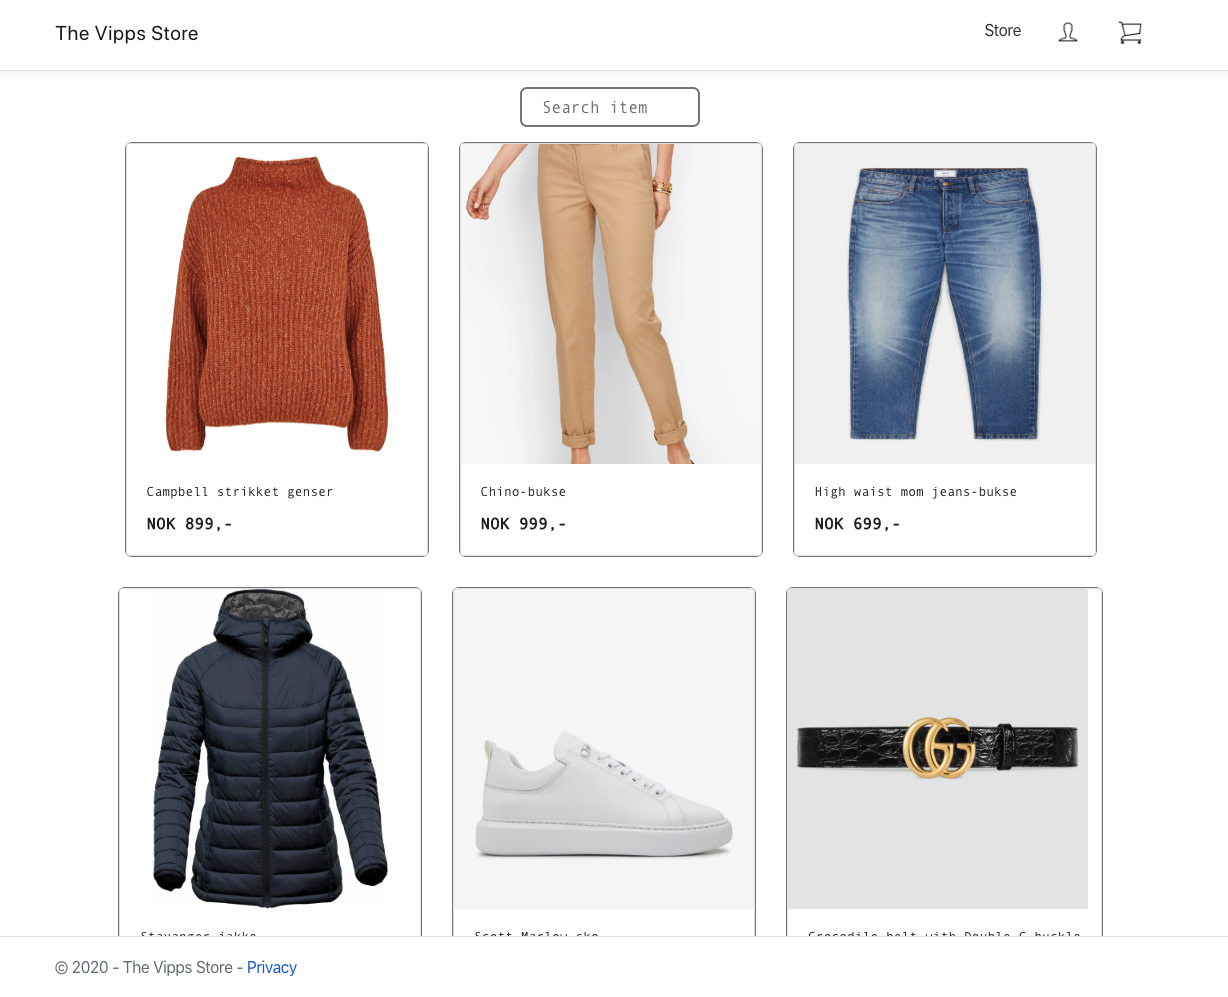
\includegraphics[scale=0.3]{home}
  \caption{Shop homepage showing products in a grid.}
  \label{fig:home}
\end{figure}
\section*{Product}
This modal opens when the product is pressed. The modal shows more information about the item and a button to add item to cart. Pressing the x in the top left corner or pressing outside of the modal closes modal, and the home page is shown again.
\begin{figure}[htbp]
  \centering
  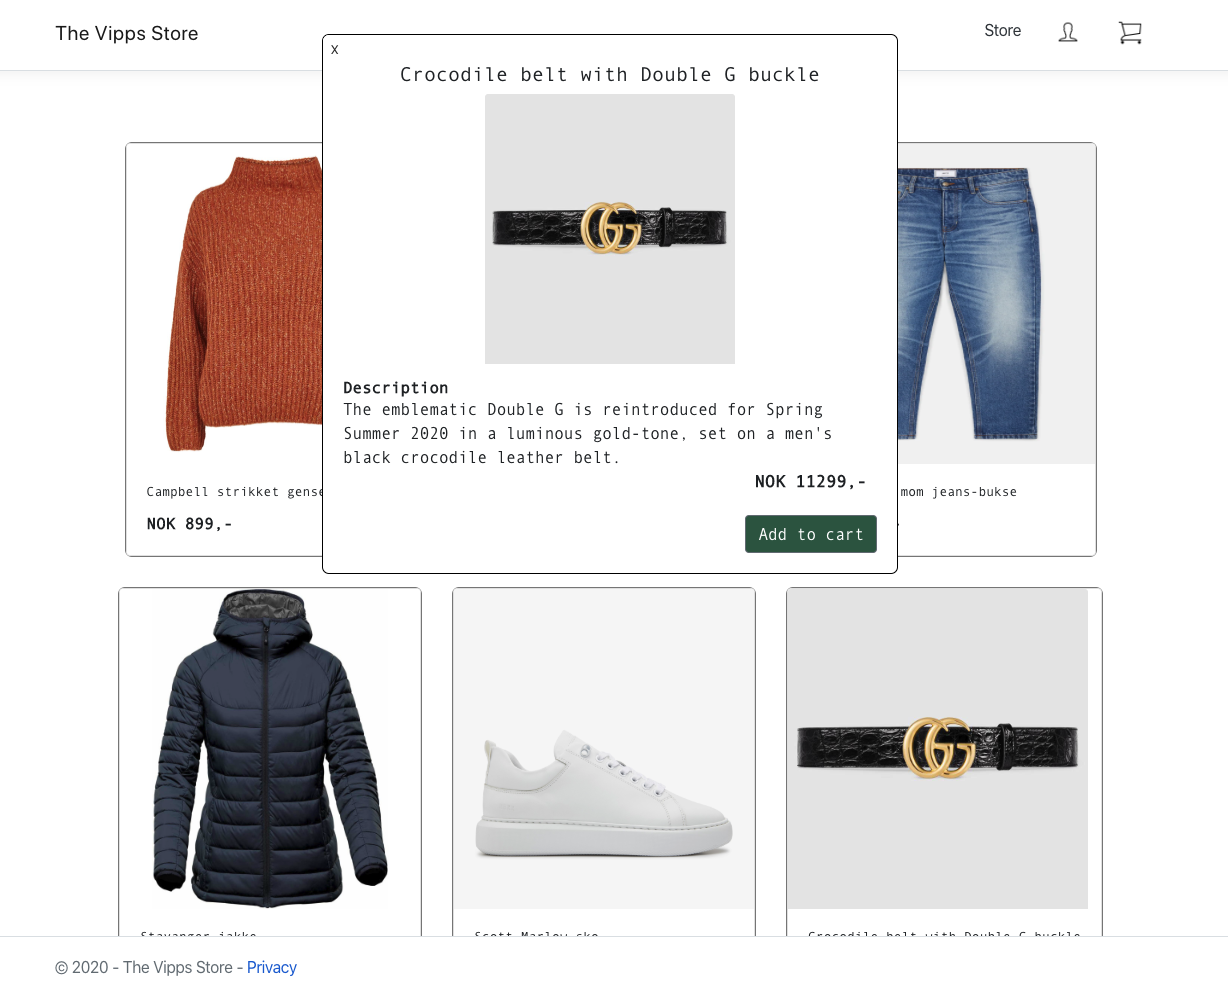
\includegraphics[scale=0.3]{item}
  \caption{Modal showing the product information.}
  \label{fig:item}
\end{figure}
\section*{Cart}
The cart page is shown in \ref{fig:cart} shows a list of the items added to cart. Each item has a button to remove the item from cart. A sum of the amount for the items added to cart is shown with a button to continue to order page.
\begin{figure}[htbp]
  \centering
  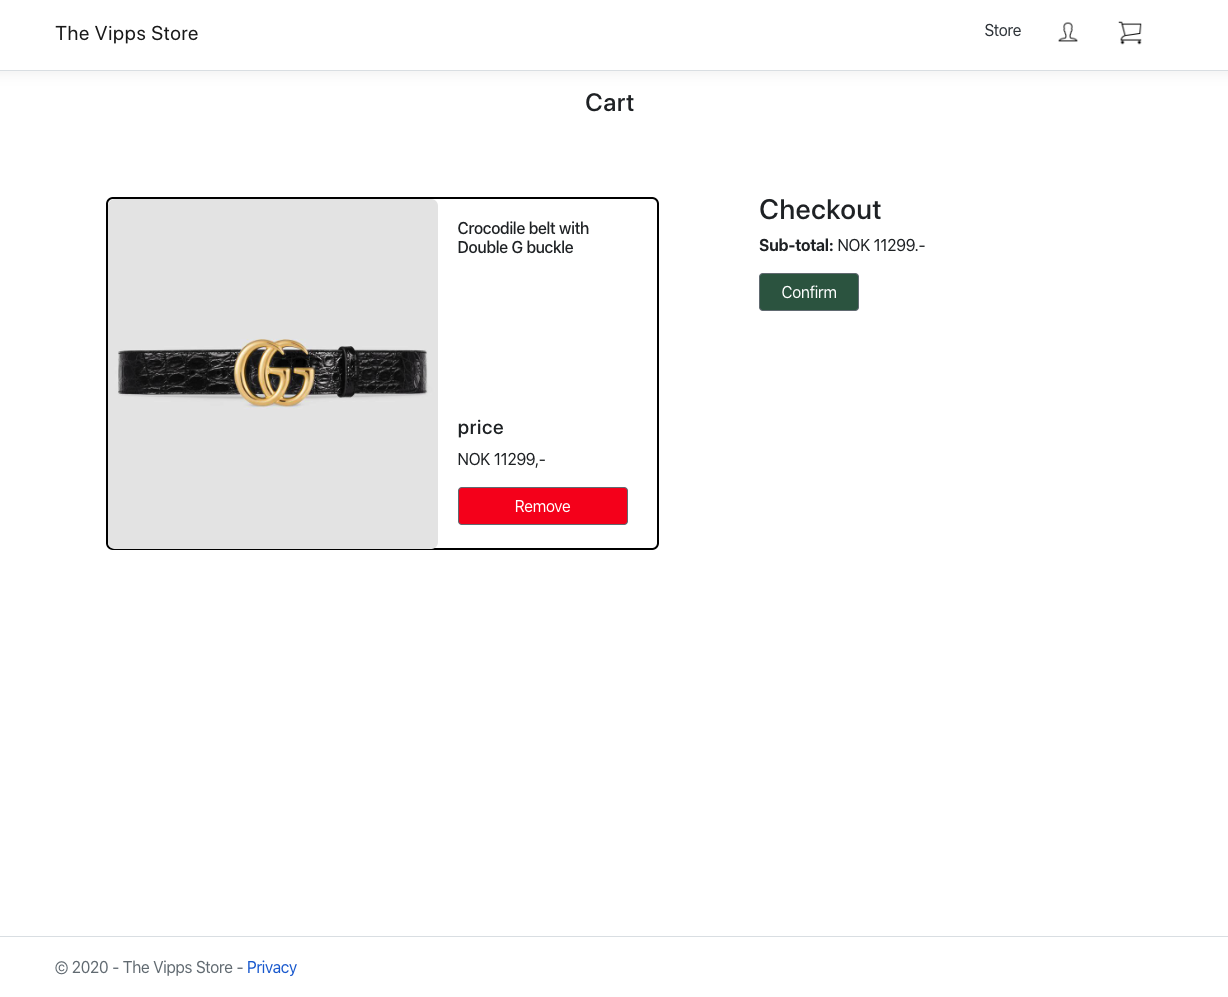
\includegraphics[scale=0.3]{cart}
  \caption{}
  \label{fig:cart}
\end{figure}

\section*{Order details}
\begin{figure}[htbp]
  \centering
  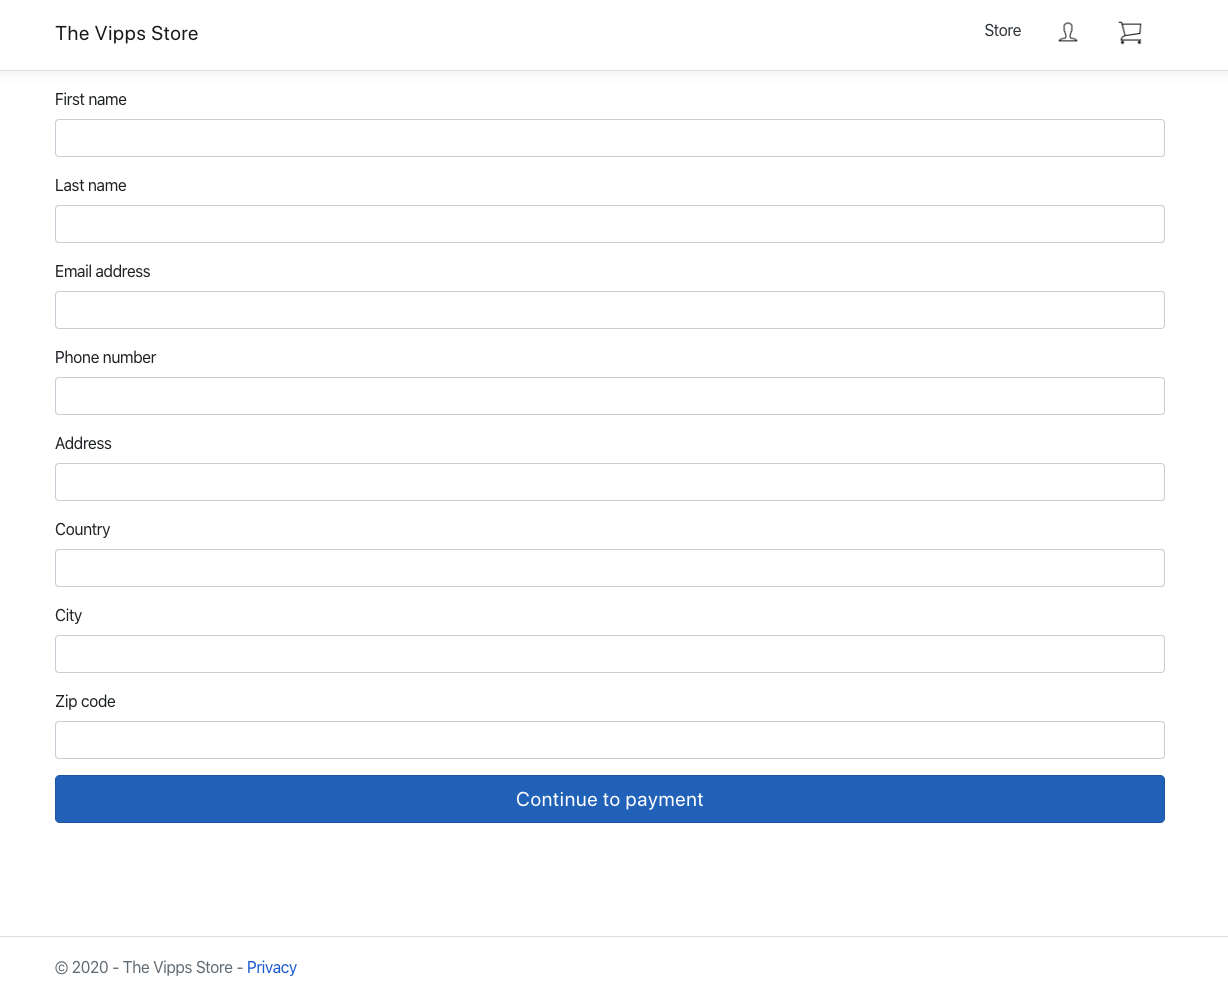
\includegraphics[scale=0.3]{order}
  \caption{}
  \label{fig:order}
\end{figure}
\end{document}
